\documentclass[final,5p,times,twocolumn]{elsarticle}
% Explicit font maps for minimal TeX installations; valid in standard TeX Live.
\pdfmapfile{+cm.map}
\pdfmapfile{+cmextra.map}
\pdfmapfile{+symbols.map}
\pdfmapfile{+txfonts.map}
\pdfmapfile{+utm.map}
\pdfmapfile{+uhv.map}
\pdfmapfile{+ucr.map}
\pdfmapline{rtxptmr NimbusRomNo9L-Regu "TeXBase1Encoding ReEncodeFont" <tx8r.enc <utmr8a.pfb}
\pdfmapline{rtxptmb NimbusRomNo9L-Medi "TeXBase1Encoding ReEncodeFont" <tx8r.enc <utmb8a.pfb}
\pdfmapline{rtxptmri NimbusRomNo9L-ReguItal "TeXBase1Encoding ReEncodeFont" <tx8r.enc <utmri8a.pfb}
\pdfmapline{rtxptmbi NimbusRomNo9L-MediItal "TeXBase1Encoding ReEncodeFont" <tx8r.enc <utmbi8a.pfb}
\pdfmapline{rtxptmro NimbusRomNo9L-Regu ".167 SlantFont TeXBase1Encoding ReEncodeFont" <tx8r.enc <utmr8a.pfb}
\pdfmapline{rtxptmbo NimbusRomNo9L-Medi ".167 SlantFont TeXBase1Encoding ReEncodeFont" <tx8r.enc <utmb8a.pfb}

\usepackage{graphicx}
\usepackage{amsmath,amssymb}
\usepackage{booktabs,array}
\usepackage{xurl}
\urlstyle{same}
\usepackage{hyperref}
\hypersetup{hidelinks}
\setcounter{dbltopnumber}{3}
\renewcommand{\dbltopfraction}{0.92}
\renewcommand{\textfraction}{0.05}
\newcommand{\pos}[1]{\left[#1\right]_+}
\journal{Robotics and Autonomous Systems}
\lefthyphenmin=3
\righthyphenmin=3
\emergencystretch=0.6em
\begin{document}
\raggedbottom
\begin{frontmatter}
\title{Preference-Conditioned Speed and Steering Control for a Single-Track Robot}
% Author and affiliation details are to be supplied by the authors.
\begin{abstract}
Speed, steering and lean are coupled in a single-track robot, so following a tight path and maintaining requested speed can require different control choices. We study a task-priority interface in which a preference-conditioned middle policy jointly adjusts speed and steering above a frozen balance controller. H75 is evaluated at five preferences on four earlier routes and, with a continued policy U170 and a zero-middle pure-pursuit comparator, in a new matched matrix of 504 simulated rollouts. The matrix spans left and right turns, S turns, exact $90^\circ$ corners, three requested speeds, matched initial states and a lateral force pulse. Increasing H75's speed priority generally raises measured bend speed and original-path error. All high-speed cases enter the original goal disk, while low- and medium-speed arrival has exceptions. Pure pursuit usually tracks the original path more closely; one disturbed low-speed S-turn pair instead shows smaller path error and slightly greater speed for H75 at high speed priority. The results establish a measurable, route-dependent preference response and identify where reference allocation still needs improvement.
\end{abstract}
\begin{keyword}
Single-track robot \sep Task-priority control \sep Preference-conditioned control \sep Path tracking \sep Speed regulation \sep Reinforcement learning
\end{keyword}
\end{frontmatter}

\section{Introduction}
A single-track robot cannot treat route tracking, forward speed and balance as independent commands. Steering changes travel direction and the lateral force supporting lean; forward speed changes the lean demand associated with a turn. When the requested maneuver approaches the useful control range, preserving speed and preserving the original path may call for different reference adjustments. Destination entry alone does not show how the requested motion was executed.

Two applications illustrate the distinction. In space-constrained passage, lateral departure may be costly even when slowing is acceptable. In a turn with permitted lateral deviation, maintaining forward speed may matter more than following the centreline closely. These contexts motivate a user-selectable priority while keeping corridor limits explicit. The controller should expose that priority through measured speed and path behavior while retaining the same balance-control foundation.

Reference and command governors modify requests to respect system constraints~\cite{garone2017}; residual reinforcement learning combines learned corrections with established controllers~\cite{johannink2019}. For unmanned bicycles, Huo et al.~\cite{huo2025} study hierarchical residual path tracking at a regulated speed. Preference-conditioned multi-objective learning provides a way to share parameters across objective weights~\cite{abels2019}. We study task-level allocation between speed loss and path deviation through two reference channels. Hierarchical organization, residual correction and a frozen lower policy implement this interface; the contribution concerns preference allocation.

We use one middle policy to generate bounded, filtered corrections to both speed and steering, conditioned on a scalar preference. The original route, speed request and lower balance controller remain common when the preference changes. This permits paired experiments from the same complete state, so measured motion reveals the realized compromise.

The study formulates joint speed and steering priority control above one balance layer. Paired simulations measure how preference changes speed loss, path departure and lean on single turns, S turns and exact right-angle references. Pure pursuit with zero middle correction and a second frozen learned policy provide matched comparisons under the same lower controller.

\section{Task and control formulation}
\label{sec:problem}
\subsection{Coupled speed steering and lean demand}
Let $v$, $\delta$ and $\phi$ denote forward speed, steering angle and roll angle, respectively. For wheelbase $L$, caster angle $\beta_{\rm c}$, path curvature $\kappa$ and gravitational acceleration $g$, the low-slip steady-turn relations are
\begin{equation}
\kappa\simeq\frac{\cos\beta_{\rm c}\tan\delta}{L},\qquad
 a_y\simeq v^2\kappa,\qquad
 \tan\phi_{\rm eq}\simeq\frac{v^2\kappa}{g}.
\label{eq:coupling}
\end{equation}
At a fixed nonzero curvature, greater speed raises the lateral acceleration and equilibrium lean. Reducing speed changes both that demand and the operating point of the balance controller. Conversely, altering the steering reference changes the path and the roll reference. The objectives can therefore compete under limited control authority, but a tracking loss is not inevitable in every turn. These relations motivate joint reference adjustment; the experiments propagate the multibody model and its contact dynamics rather than the steady-turn approximation.

The prescribed route is a world-frame curve $P_0(s)$ parameterized by arc length. A rollout specifies $P_0$, a requested forward speed $v_0$ and a fixed preference $\alpha$. Projection onto the original curve gives signed cross-track error $e_y^0$, heading error $e_h^0$ and progress $s^0$. Speed error is $e_v=v-v_0$. Tracking is evaluated against this original geometry for all preferences. The preference controls how the policy allocates its speed and steering corrections; it does not change the prescribed route or requested speed used for reporting.

Locally, the lateral-acceleration demand changes approximately as
\begin{equation}
 \Delta a_y\simeq 2v\kappa\,\Delta v+v^2\Delta\kappa.
\label{eq:localallocation}
\end{equation}
This first-order steady-turn interpretation separates the influence of speed and curvature changes. It motivates two reference channels but is not a causal decomposition of the transient multibody response or proof that both channels are necessary.

The dimensionless preference enters the observation and training objective. The closed-loop response determines its physical speed--error operating point; its numerical value is not a desired tracking error or a speed setpoint.

\subsection{Hierarchical reference interface}
\begin{figure*}[t]
\centering
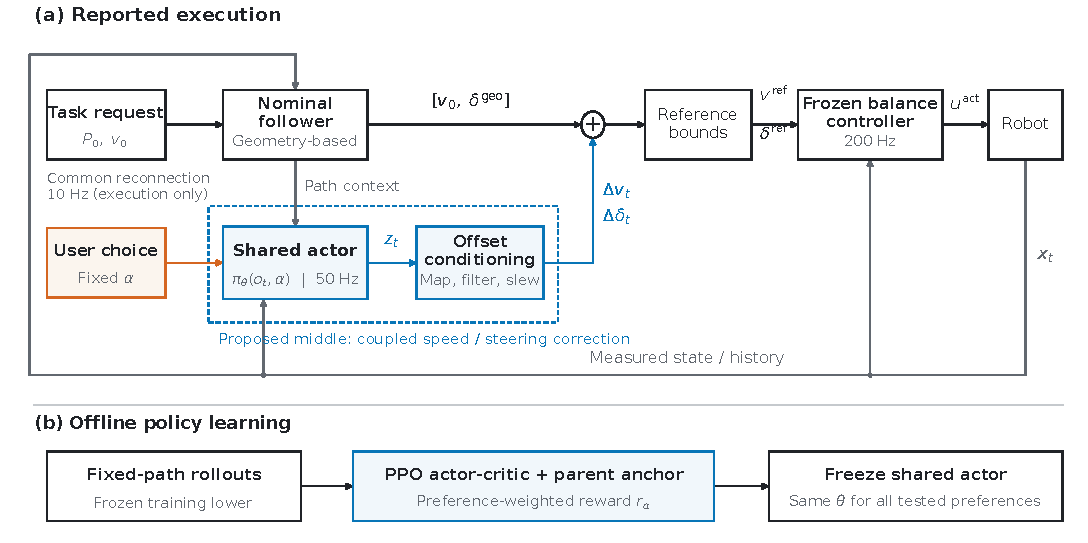
\includegraphics[width=0.98\textwidth]{figures/preference_control_architecture.pdf}
\caption{Task-priority control through a shared reference interface. A user preference conditions joint speed and steering corrections at 50~Hz, while the common frozen lower layer regulates balance at 200~Hz. The original path remains the tracking reference when the evaluation planner reconnects the execution path. The training and evaluation lower-controller configurations are distinguished.}
\label{fig:architecture}
\end{figure*}
Figure~\ref{fig:architecture} shows the hierarchy. A geometric follower supplies nominal steering, and the requested speed supplies the longitudinal reference. At 50~Hz the middle policy uses vehicle history, local route information and $\alpha$ to produce two latent outputs. Reference filtering converts these outputs to bounded speed and steering offsets. The lower layer combines conventional balance feedback, an extended-state observer and a frozen local residual policy at 200~Hz. The simulator integrates at 5~kHz.

For middle observation $o_t$, latent action $z_t$ and filter state $\eta_t$, the delivered reference is
\begin{equation}
\begin{bmatrix}v_t^{\rm ref}\\\delta_t^{\rm ref}\end{bmatrix}
=\mathcal G\!\left(v_0,\delta_t^{\rm geo},z_t,\eta_t\right),
\qquad z_t\sim\pi_\theta(\cdot\mid o_t,\alpha).
\label{eq:interface}
\end{equation}
The map $\mathcal G$ applies action scaling, low-pass filtering, slew limits and reference bounds. One parameter vector $\theta$ serves all tested preferences. During deterministic evaluation, the latent Gaussian mean is used. The preference is fixed before the rollout, with no online preference selector or policy switching.

The lower layer converts the delivered steering reference to an equilibrium roll reference. With wheel-speed estimate $v_w=r_w\omega_{\rm rear}$, disturbance estimate $\widehat d$, roll-model coefficient $a_4$ and gain schedule $K$, the conventional balance command is
\begin{equation}
\begin{split}
 \phi^{\rm ref}&=\delta^{\rm ref}/q(v_w),\\
 u_{\rm bal}&=\operatorname{clip}_{[-u_{\max},u_{\max}]}\!\left(
 K(v_w)^\top
 \begin{bmatrix}\delta^{\rm ref}-\delta\\
 \phi^{\rm ref}-\phi-\widehat d/a_4\\-\dot\phi\end{bmatrix}\right).
\end{split}
\label{eq:lowerbalance}
\end{equation}
Here $q(v)$ is the lower model's equilibrium steering-to-roll ratio. The actuator requests are
\begin{equation}
 u^{\rm act}=\mathcal A\!\left(
 \begin{bmatrix}u_{\rm bal}\\v^{\rm ref}/r_w\end{bmatrix}
 +\operatorname{clip}_{[-D,D]}(D\odot\pi_{\rm L}(o^{\rm L})),\xi^{\rm act}\right),
\label{eq:lowerresidual}
\end{equation}
where $r_w$ is wheel radius, $D$ gives residual-channel limits and $\mathcal A$ enforces actuator rate, slew and travel constraints with memory $\xi^{\rm act}$. Observer compensation follows the lower controller's physical clock. The local actor receives ten 20-field frames and ten validity masks, giving 210 inputs, and has 256--128 ELU hidden layers. It receives neither path features nor $\alpha$. The middle layer therefore changes the tracking compromise through reference commands while the lower layer retains its local balance role.

\subsection{Execution reference and tracking reference}
After a departure, a causal geometric planner constructs a connection from the measured pose to the original route. It runs at 10~Hz in the evaluation stack. If $P_k^{\rm exec}$ is the available execution path, its update has the form
\begin{equation}
P_k^{\rm exec}=\begin{cases}
P_0,&\text{before departure},\\
\mathcal D(x_{t_k},P_0),&\text{after departure},
\end{cases}\quad t_k=k\Delta_{\rm R}.
\label{eq:reconnection}
\end{equation}
The follower reads $P_k^{\rm exec}$; the reported original-path error uses $P_0$. Keeping these references separate prevents a reconnection from redefining a path departure as zero tracking error. The planner, lower controller and physical limits are common to the nominal learned-policy and geometric-rule comparisons.

During middle-policy training the path is immutable and the original lower policy remains frozen. Evaluation uses a later common lower controller and adds the reconnection mechanism. This is an integration change shared by the compared middle policies, rather than additional optimization of their weights during testing. The middle policy observes lower-control history and filter memory, so its effective dynamics depend on the integrated stack.


\subsection{Task priorities and observable execution}
For a prescribed route and requested speed, a path-priority task accepts speed loss to limit departure from the original geometry. A speed-priority task accepts deviation within an externally specified free-space envelope to reduce speed loss. In both cases, balance and physical actuator limits remain common requirements. A fixed preference $\alpha$ selects the relative priority; it does not itself specify corridor width or certify constraint satisfaction.

Requested motion, delivered references and measured motion are distinct. A smaller commanded speed need not produce smaller path error. We therefore assess actual motion and use paired motion traces to interpret the response; channel-specific causal attribution requires matched ablations.

\section{Preference-conditioned policy learning}
\label{sec:learning}
\subsection{Conditional Markov decision process}
We train the middle policy with PPO~\cite{schulman2017}. At each middle interval $\Delta_{\rm M}$, the augmented state contains the simulator state, lower-controller and observer memory, actuator and reference-filter states, path-projection and follower memory, observation history, original task clock, fixed route, requested speed, preference and disturbance-pulse schedule. The pulse schedule specifies its enable flag, amplitude, world direction and end time. The finite-horizon conditional process is
\begin{equation}
\mathcal M_\alpha=(\mathcal S,\mathbb R^2,p,r_\alpha,\gamma,\rho_0,N),
\qquad N=\lceil T/\Delta_{\rm M}\rceil.
\label{eq:mdp}
\end{equation}
The five fixed preference values lie in $[0,1]$. Here $N$ is the full original-task horizon, not the number of steps since a saved-state reset. One transition executes $\Delta_{\rm M}/\Delta_{\rm L}$ lower ticks, each containing $\Delta_{\rm L}/\Delta_{\rm phy}$ physics steps. The actor observes $o_t=h(s_t)$ rather than the complete state. Reset distribution $\rho_0$ samples uniformly from 320 complete parent-policy states, restoring their route, preference, controller memory and original task clock. The state counts at the five preferences are $(128,21,22,21,128)$; the restored preference remains fixed.

The actor has 351 inputs: sixteen 20-field history frames, sixteen validity masks and fifteen current task/control fields. These include measured roll, steering and velocities; recent commands and residuals; the observer equilibrium shift; path errors and curvature preview; requested speed; reference offsets; filter states; and $\alpha$. The critic adds the remaining-original-horizon fraction and has 352 inputs. Separate actor and critic networks use hidden widths 128--128--64 with ELU activations. Layers two and three apply learned preference-dependent feature modulation,
\begin{equation}
\begin{split}
 b_\ell&=W_\ell h_{\ell-1}+c_\ell,\\
 h_\ell&=\operatorname{ELU}\!\left([1+(2\alpha-1)g_\ell]\odot b_\ell
 +(2\alpha-1)d_\ell\right).
\end{split}
\label{eq:modulation}
\end{equation}
The actor outputs the mean of a diagonal Gaussian latent action $z_t\in\mathbb R^2$ with learned state-independent standard deviations. PPO uses the Gaussian sample and log probability before the physical action mapping; evaluation uses the mean. For $a=\tanh z$, the offset targets are
\begin{equation}
 u_v=\begin{cases}d_v^+a_v,&a_v\ge0,\\d_v^-a_v,&a_v<0,\end{cases}
 \qquad u_\delta=d_\delta^{\max}a_\delta,
\label{eq:offset}
\end{equation}
where $d_v^+$ and $d_v^-$ are positive upward and downward amplitude bounds. Filtering and slew limits precede addition to the nominal reference and clipping to delivered-reference bounds. Table~\ref{tab:interface} gives the physical and interface parameters; the archived resolved configuration specifies input scaling and the filter implementation.

\begin{table*}[t]
\centering\small\setlength{\tabcolsep}{5pt}
\caption{Physical, clock and reference-interface parameters. Reference bounds and filter settings describe middle-policy training; all nominal comparisons use a common frozen evaluation interface.}
\label{tab:interface}
\begin{tabular}{@{}llll@{}}
\toprule
Group & Parameter & Value & Unit\\
\midrule
Geometry & Wheelbase $L$; wheel radius $r_w$; caster $\beta_{\rm c}$ & 0.408; 0.10; 25 & m; m; deg\\
Clocks & $\Delta_{\rm phy}$; $\Delta_{\rm L}$; $\Delta_{\rm M}$ & 0.2; 5; 20 & ms\\
 & Reconnection $\Delta_{\rm R}$; horizon $N$; deadline $T$ & 0.10; 500; 10 & s; steps; s\\
Offset amplitudes & $d_v^-$; $d_v^+$; $d_\delta^{\max}$ & 1.00; 0.25; 0.20 & m/s; m/s; rad\\
Filters & $\tau_v$; $\tau_\delta$ & 0.10; 0.08 & s\\
Offset slew & $\dot d_v^-$; $\dot d_v^+$; $\dot d_\delta^{\max}$ & 1.00; 0.50; 0.80 & m/s$^2$; m/s$^2$; rad/s\\
Delivered references & $v_{\min}$; $v_{\max}$; $\delta_{\max}^{\rm ref}$ & 1.50; 3.50; 0.35 & m/s; m/s; rad\\
Geometric rule & Preview length $\ell_\kappa$; lateral cap $a_{\max}$ & 6.0; 3.5 & m; m/s$^2$\\
\bottomrule
\end{tabular}
\end{table*}

\subsection{Preference-weighted reward}
Define the dimensionless robust cost $H(x)=x^2$ for $|x|\le1$ and $H(x)=2|x|-1$ otherwise, and component clipping $B_c(x)=\min(x,c)$ for $x\ge0$. Errors refer to the fixed training path and requested speed. A curvature-demand gate reduces the path-priority speed penalty during demanding turns:
\begin{equation}
 \chi=\operatorname{clip}_{[0,1]}\!\left(
 \frac{|\arctan(L\kappa/\cos\beta_{\rm c})/q(v_0)|-\phi_\chi}{\sigma_\chi}\right).
\label{eq:gate}
\end{equation}
Let $w_v(\chi)=(1-\chi)w_v^{\rm s}+\chi w_v^{\rm t}$ interpolate the straight and turning speed-cost weights. The speed, path and endpoint-band costs at a lower tick are
\begin{align}
C_v={}&(1-\alpha)B_{\bar C_v}\big(w_v(\chi)H(e_v/\sigma_v)\big)\notag\\
 &+\alpha B_{\bar C_v}\big(w_v^{\rm s}H(e_v/\sigma_v)\big),\label{eq:cv}\\
C_p={}&[1-(1-\rho_p)\alpha]B_{\bar C_p}\big(w_p[H(e_y/\sigma_y)\notag\\
 &\hspace{32mm}+w_hH(e_h/\sigma_h)]\big),\label{eq:cp}\\
C_b={}&(1-\alpha)B_{\bar C_b}\big(w_b\chi H(\pos{|e_y|-b_y}/\sigma_{by})\big)\notag\\
 &+\alpha B_{\bar C_b}\big(w_b\chi H(\pos{|e_v|-b_v}/\sigma_{bv})\big).
\label{eq:cb}
\end{align}
Each endpoint channel is capped \emph{before} preference mixing. At low $\alpha$, path and lateral-band penalties remain strong while the speed penalty relaxes with curvature demand. At high $\alpha$, the requested-speed and speed-band penalties dominate the preference-dependent allocation. Table~\ref{tab:rewardparams} lists the weights and principal scales.

\begin{table*}[t]
\centering\small\setlength{\tabcolsep}{5pt}
\caption{Reward hyperparameters used by the main policy. Weights and component costs are dimensionless; each error is divided by a physical scale. Auxiliary deadbands, scales and component caps are fixed in the archived configuration.}
\label{tab:rewardparams}
\begin{tabular}{@{}llll@{}}
\toprule
Group & Parameters & Values & Units\\
\midrule
Tracking weights & $w_v^{\rm s}$; $w_v^{\rm t}$; $w_p$; $w_h$; $w_b$ & 10; 1; 10; 0.5; 20 & --\\
Path retention & $\rho_p$ & 0.10 & --\\
Tracking scales & $\sigma_v$; $\sigma_y$; $\sigma_h$ & 0.10; 0.10; 0.10 & m/s; m; rad\\
Demand gate & $\phi_\chi$; $\sigma_\chi$ & 0.18; 0.12 & rad\\
Endpoint deadbands & $b_y$; $b_v$ & 0.10; 0.05 & m; m/s\\
Endpoint scales & $\sigma_{by}$; $\sigma_{bv}$ & 0.10; 0.10 & m; m/s\\
Roll weights & $w_\phi$; $w_w$; $w_{\dot\phi}$ & 80; 240; 1 & --\\
Speed / correction weights & $w_o$; $w_l$; $w_d$; $w_{\dot d}$ & 2; 4; 0.02; 0.03 & --\\
Reward conversion & $\lambda_r$; $C_{\rm fail}$; $C_{\max}$ & 0.10; 5; 8980.2 & s$^{-1}$; --; --\\
\bottomrule
\end{tabular}
\end{table*}

The remaining terms penalize roll excursions, roll rate, overspeed, low speed and reference corrections. For $j\in\{\phi,w,\dot\phi,o,l\}$ they have the common form
\begin{equation}
 C_j=B_{\bar C_j}\!\left(w_j H\!\left(\frac{\pos{x_j-b_j}}{\sigma_j}\right)\right),
\label{eq:auxcost}
\end{equation}
where $(x_\phi,x_w,x_{\dot\phi},x_o,x_l)=(\phi_{\rm pk},\phi_{\rm pk},|\dot\phi|,e_v,-v)$ and $\phi_{\rm pk}$ is peak absolute roll over the lower tick's physics substeps. The low-speed threshold $b_l$ is negative, so $\pos{x_l-b_l}=\pos{v_l-v}$ with $v_l=-b_l$. For applied offsets $d=(d_v,d_\delta)$, the remaining two costs are
\begin{align}
 C_d&=B_{\bar C_d}\!\left(w_d\sum_{k\in\{v,\delta\}}(d_k/\sigma_{d,k})^2\right),\\
 C_{\dot d}&=B_{\bar C_{\dot d}}\!\left(w_{\dot d}\sum_{k\in\{v,\delta\}}(\dot d_k/\sigma_{\dot d,k})^2\right),
\end{align}
where $\dot d=(d_{t+1}-d_t)/\Delta_{\rm M}$. The same offset-rate cost is assigned to each active lower tick in that middle interval.

Let $\mathcal C=\{v,p,b,\phi,w,\dot\phi,o,l,d,\dot d\}$ index the ten costs and $\mathcal A_t$ the active lower ticks. The ordinary reward and a uniform bound on total running cost are
\begin{equation}
 r_t=-\lambda_r\Delta_{\rm L}\sum_{j\in\mathcal A_t}\sum_{i\in\mathcal C}C_{i,j},
 \qquad C_{\max}=\sum_{i\in\mathcal C}\bar C_i.
\label{eq:reward}
\end{equation}
There is no additional global clipping. Write $\tau_t$ for original task time (original lower-tick count times $\Delta_{\rm L}$) at the start of a transition, and $n_t=\lfloor\tau_t/\Delta_{\rm M}\rfloor$ for its original middle-step index. Physical failure or tracking-domain exit replaces the entire failing interval's reward with
\begin{equation}
 r_t^{\rm fail}=-C_{\rm fail}-\lambda_r\Delta_{\rm M}C_{\max}
 \frac{1-\gamma^{N-n_t}}{1-\gamma}.
\label{eq:terminal}
\end{equation}
The exponent includes the failing interval and the remaining original-task intervals. Saved-state resets preserve $\tau_t$; they do not restart this horizon. The domain check includes a preview behind the vehicle or $|e_h|\ge\pi/2$. These events and finite-horizon completion terminate without value bootstrap; an unfinished episode at a rollout-buffer boundary bootstraps.

\subsection{PPO objective and training settings}
For critic input $\widetilde o_t=(o_t,1-\tau_t/T)$ and nonterminal mask $m_t$, generalized advantage estimation uses
\begin{align}
 \varepsilon_t^{\rm TD}&=r_t+\gamma m_tV_{\psi_{\rm old}}(\widetilde o_{t+1})
             -V_{\psi_{\rm old}}(\widetilde o_t),\\
 A_t&=\varepsilon_t^{\rm TD}+\gamma\lambda m_tA_{t+1},\qquad
 R_t=A_t+V_{\psi_{\rm old}}(\widetilde o_t).
\end{align}
Advantages are standardized over the rollout. With likelihood ratio $\rho_t=\pi_\theta(z_t\mid o_t,\alpha)/\pi_{\theta_{\rm old}}(z_t\mid o_t,\alpha)$, the minimized objective is
\begin{equation}
\begin{split}
\mathcal L={}&-\mathbb E\!\left[\min\!\left(\rho_t\widehat A_t,
 \operatorname{clip}(\rho_t,1-\epsilon,1+\epsilon)\widehat A_t\right)\right]\\
 &+c_V\mathbb E\!\left[(R_t-V_\psi(\widetilde o_t))^2\right]
 -c_H\mathbb E[\mathcal H(\pi_\theta)]\\
 &+\beta_{\rm anchor}\mathbb E_{o\sim\mathcal B_A}\!\left[D_{\rm KL}(\pi_{\rm parent}(\cdot\mid o)\Vert\pi_\theta(\cdot\mid o))\right].
\end{split}
\label{eq:ppo}
\end{equation}
The critic loss is not clipped. The final term anchors nominal behavior using 512 records per minibatch from a fixed bank of 25,573 parent observation/distribution records. No temporal auxiliary loss is used. A soft KL limit stops further epochs; a hard limit rejects the latest epoch and reduces the actor learning rate. Table~\ref{tab:ppo} gives the final-stage settings.

\begin{table}[t]
\centering\small\setlength{\tabcolsep}{4pt}
\caption{Final-stage PPO hyperparameters. All entries are dimensionless unless a unit is shown.}
\label{tab:ppo}
\begin{tabular}{@{}ll@{}}
\toprule
Setting & Value\\
\midrule
Environments; rollout length & 512; 128 middle steps\\
Transitions per rollout & 65,536\\
Minibatch size; epochs & 16,384; 4\\
Discount $\gamma$; GAE $\lambda$ & 0.997; 0.99\\
Policy clip $\epsilon$ & 0.2\\
Value $c_V$; entropy $c_H$ & 1; 0.001\\
Parent anchor $\beta_{\rm anchor}$ & 0.05\\
Actor; critic learning rate & $3\!\times\!10^{-5}$; $3\!\times\!10^{-4}$\\
Adam $(\beta_1,\beta_2)$; $\varepsilon_{\rm Adam}$ & $(0.9,0.999)$; $10^{-5}$\\
Weight decay; gradient norms & 0; 1 per network\\
Latent standard-deviation bounds & $[0.05,0.5]$\\
Soft/hard mean KL & 0.01/0.03\\
Training; pulse-sampling seed & 918301; 918203\\
\bottomrule
\end{tabular}
\end{table}

The final stage starts from a shared actor and critic obtained by endpoint-policy distillation and curriculum PPO. It performs two critic-only collections and 75 PPO collections, totaling 5,046,272 collected transitions, including 4,915,200 in PPO collections. These counts describe one final training stage. Complete states captured at original task times of 0.8--3.5~s continue to the original deadline $T$. Independently at each reset, a lateral pulse is enabled with probability 0.8, lasts 0.1~s and has uniformly sampled signed amplitude in $\{\pm8,\pm16,\pm24,\pm32\}$~N. Its direction is perpendicular to the captured heading and fixed in world coordinates. The original lower controller remains frozen and training paths are immutable. The common evaluation lower controller and causal reconnection are introduced only at evaluation. The final actor and critic parameters, resolved training configuration and training logs are archived with the run.


\section{Experimental questions and measurement}
\label{sec:experiments}
\subsection{Questions linked to the task priorities}
The experiments address three questions. Does changing preference under a common request produce a consistent change in actual speed and original-path deviation? How does that response vary with turn geometry and relative to a controller without middle correction? What does the available evidence establish about space-constrained and speed-preserving turning tasks? We distinguish a nominal multi-route comparison from earlier trajectory examples so that qualitative mechanism illustrations do not become additional test repetitions.

For task-level assessment, the intended primary measurements are mean actual speed and mean absolute and root-mean-square original-path error over a common bend segment. Maximum excursion and peak lean complement these averages. Space-constrained passage additionally requires a specified admissible corridor; speed-preserving turning requires a declared permissible deviation envelope. Neither context should be ranked solely by arrival within an arbitrary observation window.

\subsection{Available continuous quantities}
The available nominal tables report mean actual turn speed and the mean of episode-wise maximum absolute original-path error before destination entry. For episode $n$, the latter is
\begin{equation}
 M_n=\max_{0\le t<\min(t_{g,n},T_{\rm obs})}|e_{y,n}^0(t)|,
 \qquad \overline M=\frac1{N_{\rm ep}}\sum_{n=1}^{N_{\rm ep}} M_n.
\label{eq:maxerror}
\end{equation}
Here $t_g$ is first entry into the original destination disk and $T_{\rm obs}=10$~s is the recording horizon, not the task objective. Arrival and upright survival are validity information rather than the performance ranking. The exact sample mask of the older stored turn-speed statistic is unavailable; grouped peak errors cannot recover MAE or RMSE. We report those quantities as stored. The new matched matrix below uses raw trajectories and computes original-path MAE and RMSE directly over a declared bend-vicinity segment.

\subsection{Nominal routes and paired states}
Table~\ref{tab:routes} gives the four nominal route--speed combinations. Each uses two matched complete initial states, including simulator and controller memory. The same learned policy is evaluated at $\alpha\in\{0,0.25,0.5,0.75,1\}$ in each context, giving 40 episodes. The geometric rule runs once per context, giving eight episodes. Nominal wheel sliding friction is 0.8 in the MuJoCo model~\cite{todorov2012}. Route means pool the two states; aggregate means weight the four routes equally.
\begin{table}[t]
\centering\small
\caption{Nominal route--speed combinations. Each uses the same two complete initial states across preferences and controllers.}
\label{tab:routes}
\begin{tabular}{@{}lrrr@{}}
\toprule
Route & Angle & Radius (m) & $v_0$ (m/s)\\
\midrule
Low single left & $76^\circ$ & 1.45 & 1.90\\
Low S right & $72^\circ$ & 1.55 & 2.00\\
High single right & $96^\circ$ & 3.15 & 3.05\\
High S left & $70^\circ$ & 3.10 & 3.10\\
\bottomrule
\end{tabular}
\end{table}
These prepared states are not independent training seeds. The comparison contains one trained realization of the preference-conditioned policy and is not an independently locked task-validation study. A later low-speed continuation supplied the U170 comparison actor; it is assessed separately in the new matched route matrix.

\subsection{Reference-controller comparisons}
The nominal geometric comparator retains pure-pursuit steering~\cite{coulter1992}, common reference conditioning, the frozen evaluation lower layer, actuator limits and 10~Hz reconnection. It removes the learned middle correction and uses
\begin{equation}
 v_{\rm rule}=\min\!\left(v_0,\sqrt{\frac{a_{\max}}{\max_{s\in[s_t,s_t+\ell_\kappa]}|\kappa(s)|}}\right),
\label{eq:rule}
\end{equation}
with straight-path limit $v_0$. Curvature is read from the execution path. The lateral-acceleration cap $a_{\max}=3.5$~m/s$^2$ was selected from $\{1.5,2.5,3.5,5.0\}$ on development routes and fixed for this comparison. The rule was introduced after inspecting the learned outcomes, so its nominal result is a descriptive reference rather than a blind confirmation result. Because it shares the learned lower balance controller, this comparison tests the middle reference strategy rather than learning versus no learning anywhere in the system.

\subsection{Matched speed, geometry and disturbance matrix}
The extended matrix uses six routes at each of three requested speeds: 1.90, 2.50 and 3.05~m/s. Each speed stratum includes left and right single turns and left- and right-leading S turns; the low and high strata also contain a tighter single-turn pair. The medium stratum contains two exact $90^\circ$ polyline corners, one left and one right. These corner references change heading discontinuously at the vertex: no clothoid, circular arc, or curvature-based rounding is inserted. The vehicle may round the corner in its actual motion. Every original destination is 7~m after the last bend or vertex, with a 1~m arrival disk.

For each route we restore two complete prepared initial states, then run the fixed H75 policy at $\alpha\in\{0,0.5,1\}$, a second frozen learned middle policy U170 at the same preferences, and a pure-pursuit reference follower with exactly zero middle correction. U170 continues H75 with two critic-only collections and 168 PPO updates over a mixture that includes low-speed tight turns; it is not an independently initialized training seed. Each controller has a nominal run and a run with a $+36$~N world-Y force applied from 2.80 to 2.95~s. Thus the declared matrix contains $18\times2\times2\times7=504$ physical rollouts, each with a 10~s observation window. All controllers share the same lower layer, vehicle model with 0.8 nominal wheel sliding friction, actuator constraints, reference conditioning and 10~Hz causal reconnection. A force applied in a fixed world direction need not have the same body-lateral sign after left and right turns.

The matrix was designed after inspection of earlier development cases, and H75 was previously selected as the main policy. It is therefore an exploratory matched comparison, not independent confirmation. The evaluation uses 0.8 sliding friction at both wheels, whereas the historical H75 training identity used a different front-wheel contact setting; this is a common evaluation-domain change, not a single-factor friction study. We retain all route--state--event outcomes in the accompanying per-case record. Bend speed and original-path MAE are computed from raw measured trajectories in a common original-progress region spanning the turn and 2~m beyond it. Arrival, contact failure, controller fault and full-horizon completion are reported separately; arrival does not by itself imply accurate sustained tracking.

\section{Results}
\label{sec:results}
\subsection{What user preference changes across turns}
Figure~\ref{fig:tradeoff} addresses the central execution question: under the same route and speed request, how much actual speed is retained and how far does the robot depart from the original path as preference changes? Across the four nominal routes, increasing $\alpha$ from 0 to 1 raises mean turn speed from 2.200 to 2.458~m/s and mean maximum pre-arrival path error from 0.223 to 0.615~m (Table~\ref{tab:nominal}). The same network therefore exposes distinct physical operating points, rather than only distinct reward labels.
\begin{figure*}[t]
\centering
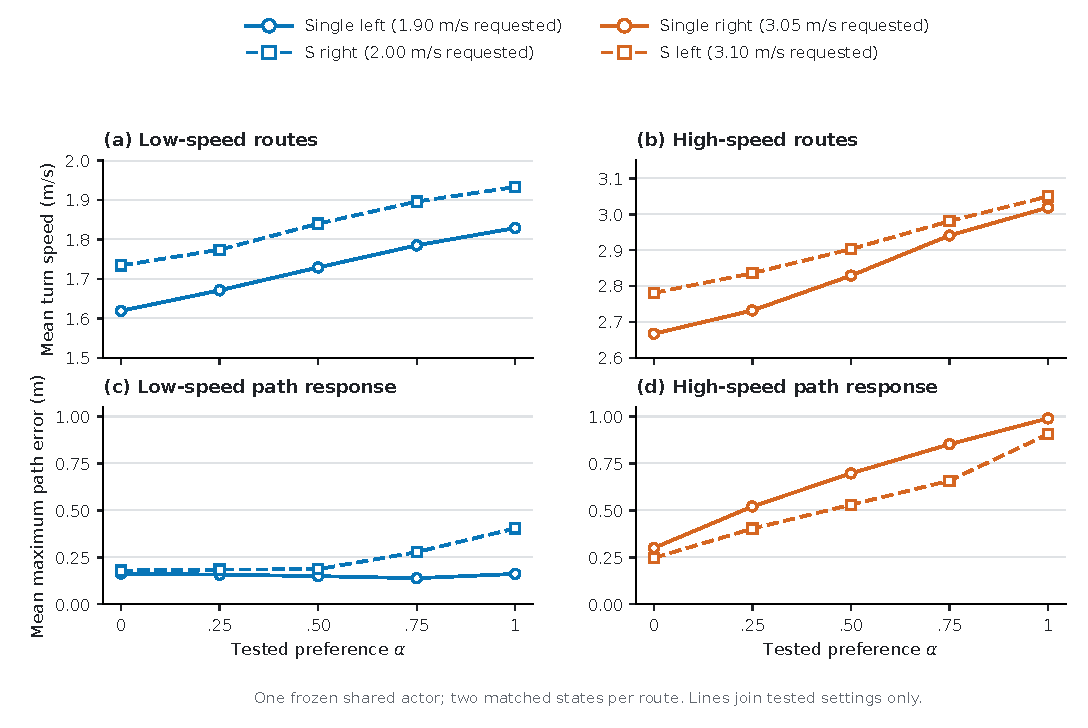
\includegraphics[width=0.98\textwidth]{figures/h75_route_preference_evidence.pdf}
\caption{How preference changes actual execution on multiple routes. Route-resolved curves show stored mean turn speed and mean episode-wise maximum original-path error before arrival, each averaged over two matched complete initial states. Table~\ref{tab:nominal} retains the geometric curvature-speed comparator at the aggregate level. The error is a peak statistic, not MAE or RMSE; lines connect tested preferences and do not establish continuous interpolation.}
\label{fig:tradeoff}
\end{figure*}
\begin{table}[t]
\centering\small
\caption{Nominal continuous outcomes. Every row averages eight matched route--state contexts. Intermediate policy aggregates use route means rounded to three decimals.}
\label{tab:nominal}
\begin{tabular}{@{}lrr@{}}
\toprule
Controller / preference & Speed (m/s) & Maximum error (m)\\
\midrule
Preference policy, $\alpha=0$ & 2.200 & 0.223\\
Preference policy, $\alpha=0.25$ & 2.253 & 0.317\\
Preference policy, $\alpha=0.50$ & 2.325 & 0.391\\
Preference policy, $\alpha=0.75$ & 2.401 & 0.482\\
Preference policy, $\alpha=1$ & 2.458 & 0.615\\
Geometric rule & 2.469 & 0.233\\
\bottomrule
\end{tabular}
\end{table}

The response depends strongly on the route. On the high-speed single right turn, speed increases from 2.667 to 3.019~m/s while mean maximum error increases from 0.300 to 0.990~m. On the high-speed S left turn, the corresponding changes are 2.781 to 3.050~m/s and 0.247 to 0.906~m. Moving toward the requested speed on these routes is accompanied by substantially larger lateral excursions.

The low-speed S right turn shows a smaller exchange: speed rises from 1.734 to 1.933~m/s and error from 0.180 to 0.404~m. The low-speed single left turn is an important exception. Speed rises from 1.619 to 1.829~m/s, while endpoint errors are almost equal, 0.164 and 0.162~m; the error at $\alpha=0.75$ is lower still, at 0.139~m. Thus, changing priority does not enforce a monotone path-error response, and better speed need not always require worse tracking.

These outcomes support a route-dependent priority interface. They do not show an unavoidable physical tradeoff or an optimal allocation. The high- and low-speed strata also differ in geometry and turn direction, so their contrast does not isolate requested speed as the only causal factor.

\subsection{Response to a lateral pulse on a low-speed S turn}
Figure~\ref{fig:pulse} shows an illustrative pair of complete-state banks on a low-speed left-leading S turn. The pulse is identical in world coordinates for every controller in each bank. With $\alpha=1$, H75 enters the original destination region in both banks. Its bend speed is 1.909 and 1.912~m/s, compared with 1.892 and 1.889~m/s for pure pursuit; original-path bend MAE is 0.221 and 0.151~m, compared with 0.375 and 0.237~m. Peak excursions are 0.427 and 0.275~m, compared with 1.150 and 1.226~m. Neither controller records contact failure in these cases. This is a positive disturbance example for the learned interface, selected after viewing the exploratory matrix rather than an estimate of a population-wide effect.
\begin{figure*}[t]
\centering
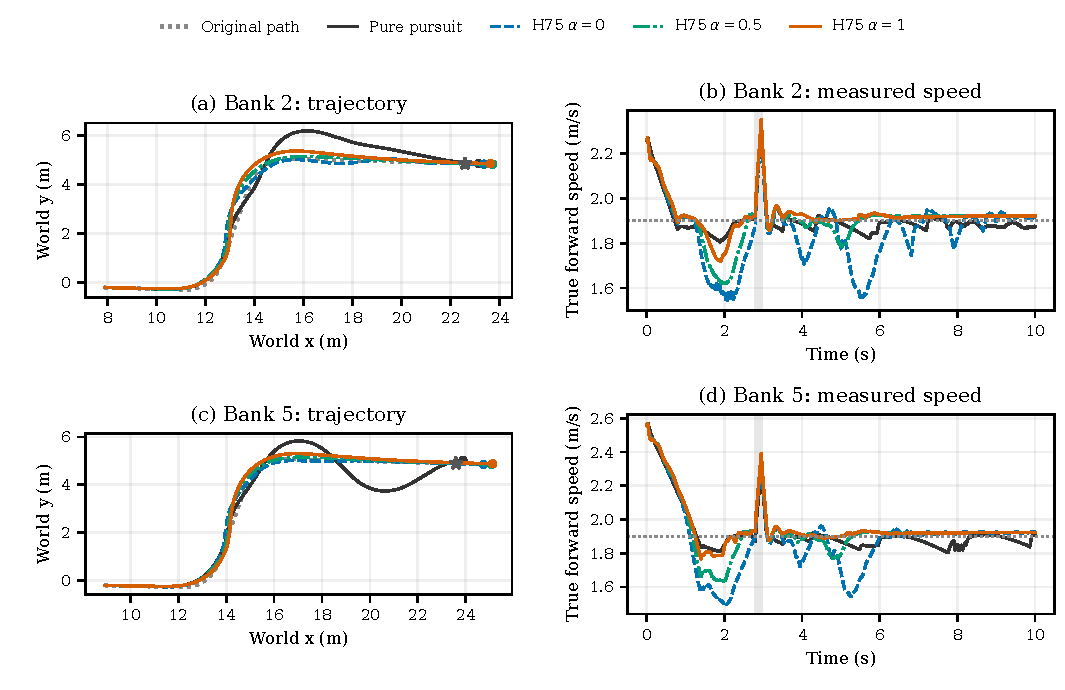
\includegraphics[width=0.98\textwidth]{figures/low_s_pulse_matched.pdf}
\caption{Matched actual XY trajectories and measured forward speed for the two prepared states on the 1.90~m/s left-leading S turn, with a $+36$~N world-Y pulse over 2.80--2.95~s (gray band). Dotted black/gray denotes the original path and requested speed, not an execution-path reset. The star marks the original goal 7~m beyond the last bend; endpoint markers show actual final positions. All four controllers reach the goal without contact failure in these two cases. The selected example is exploratory; the complete route matrix is reported separately.}
\label{fig:pulse}
\end{figure*}

Under zero pulse on this same route, pure pursuit has lower bend MAE than H75 at $\alpha=1$ in both banks (0.071 versus 0.134~m and 0.070 versus 0.133~m). Thus the disturbance example does not imply that H75 dominates the geometric follower in nominal tracking. The matched contrast instead shows one setting in which the learned reference response reduces a perturbation-induced departure while retaining speed.

\subsection{An unsmoothed right-angle reference}
Figure~\ref{fig:sharp} compares actual motion against the two exact polyline corners. The original reference goes straight for 5~m and changes heading by $90^\circ$ at one vertex; it is not a circular or curvature-smoothed target. Both directions use a goal 7~m after the vertex. The traces expose how each controller negotiates a discontinuous geometric request; a rounded actual trajectory is expected from finite steering and lean dynamics and must not be mistaken for a rounded input path.
\begin{figure*}[t]
\centering
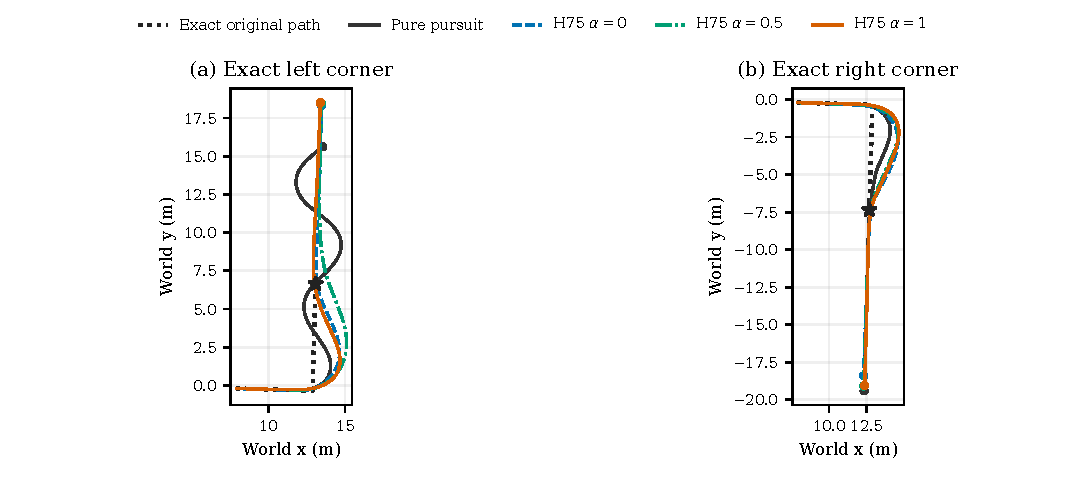
\includegraphics[width=0.98\textwidth]{figures/exact_sharp90_matched.pdf}
\caption{Actual XY trajectories from state bank 2 at 2.50~m/s, compared with exact left and right $90^\circ$ polyline references (dotted). The reference has no inserted curved segment. The star marks the original goal 7~m after the corner, circles indicate final positions after destination entry, and crosses indicate an episode ending without that entry. H75 uses three fixed preferences; pure pursuit has zero learned middle correction. All raw trajectories, including the second state bank and disturbed corners, are retained in the matrix inventory.}
\label{fig:sharp}
\end{figure*}

\subsection{Complete matched route matrix}
Table~\ref{tab:matrix} reports all speed strata and both force conditions; each cell aggregates six route geometries and two complete prepared states. The high-speed stratum reaches the original goal disk in every case for all seven controllers. At 1.90~m/s under the force pulse, H75 reaches in 10, 11 and 12 of 12 cases as $\alpha$ increases from 0 to 1; U170 has the same entry counts, and pure pursuit reaches in 12. At 2.50~m/s without the pulse, H75 at $\alpha=1$ reaches in 11 of 12, whereas U170 at $\alpha=0.5$ and 1 reaches in 10 of 12. All medium-speed pulse cases enter the goal disk. No case in the matrix is marked as a contact failure or controller fault; non-arrival and contact failure are distinct outcomes.

Across all three speeds, H75's average measured bend speed rises with $\alpha$. Its mean original-path bend MAE also rises in five of the six speed--force strata; in the disturbed low-speed stratum the three values are 0.271, 0.259 and 0.343~m. The geometric comparator has lower bend MAE than every H75 setting in the medium and high strata, and in both nominal and disturbed low-speed aggregate rows. Thus the learned controller's observable preference response is stronger evidence here than absolute tracking superiority. U170 is not consistently better than H75 despite its additional training; we retain it as a distinct learned outcome rather than replacing the selected main policy.

\begin{table*}[t]
\centering\scriptsize\setlength{\tabcolsep}{4pt}
\caption{Complete matched route-matrix summary. Each cell gives original-goal entries (out of 12); mean measured bend speed (m/s) / mean original-path bend MAE (m). Each speed--event cell comprises six routes and two complete initial states; no model is trained in this evaluation. All 504 physical trajectories and per-case metrics are retained.}
\label{tab:matrix}
\begin{tabular}{@{}llccccccc@{}}
\toprule
Speed & Force & PP & H75 $\alpha=0$ & H75 $\alpha=.5$ & H75 $\alpha=1$ & U170 $\alpha=0$ & U170 $\alpha=.5$ & U170 $\alpha=1$\\
\midrule
1.90 & 0 & 12;1.874/0.071 & 12;1.786/0.079 & 12;1.849/0.083 & 12;1.894/0.153 & 12;1.712/0.117 & 12;1.753/0.131 & 12;1.811/0.154\\
1.90 & $+36$ N & 12;1.879/0.233 & 10;1.771/0.271 & 11;1.854/0.259 & 12;1.902/0.343 & 10;1.677/0.378 & 11;1.746/0.342 & 12;1.818/0.320\\
\addlinespace[2pt]
2.50 & 0 & 12;2.443/0.327 & 12;2.279/0.388 & 12;2.413/0.459 & 11;2.467/0.549 & 12;2.171/0.402 & 10;2.281/0.476 & 10;2.392/0.545\\
2.50 & $+36$ N & 12;2.451/0.369 & 12;2.291/0.435 & 12;2.423/0.511 & 12;2.478/0.587 & 12;2.167/0.499 & 12;2.283/0.563 & 12;2.400/0.594\\
\addlinespace[2pt]
3.05 & 0 & 12;2.999/0.076 & 12;2.790/0.109 & 12;2.899/0.251 & 12;3.013/0.435 & 12;2.710/0.196 & 12;2.794/0.261 & 12;2.907/0.363\\
3.05 & $+36$ N & 12;3.003/0.125 & 12;2.787/0.158 & 12;2.906/0.320 & 12;3.025/0.492 & 12;2.694/0.205 & 12;2.786/0.278 & 12;2.918/0.400\\
\bottomrule
\end{tabular}
\end{table*}


\subsection{Comparison with a geometric speed allocation}
The geometric rule reaches 2.469~m/s mean turn speed with 0.233~m mean maximum pre-arrival error. It is faster and has lower aggregate error than every learned setting with $\alpha\ge0.25$. At $\alpha=0$, the learned controller has 0.010~m less error but is 0.269~m/s slower. The small error difference is descriptive and does not establish superiority with only two initial states and one trained realization.

The rule separates adjustability from the quality of the operating points. The larger learned deviations cannot be attributed solely to physical coupling: better reference allocation is possible on these routes. This earlier rule also differs from the new matrix comparator, which uses pure pursuit with zero middle correction and no curvature-speed cap. A future locked comparison should test error at matched measured speed.

\section{Task interpretation and remaining validation}
For space-constrained passage, the path-priority endpoint is a plausible operating choice when slowing is acceptable, because its nominal aggregate excursions are smaller. For a turn with permitted deviation, increasing speed priority generally preserves more of the requested speed. These are interpretations of the observed response, not demonstrations that a particular corridor was traversed within its boundaries or that a specified speed-retention requirement was met. Such requirements must be fixed before the corresponding task test.

A complete mechanism experiment should hold the full initial state, route and request constant, compare joint correction with unmodified-reference, speed-only and steering-only control, and record both requested and delivered references. It should include low-demand and high-demand maneuvers so that channel use can be related to the speed--steering--lean demand rather than selected from a single favorable example. Training separate restricted-channel policies is distinct from disabling one channel at evaluation; both interventions answer useful but different questions.

The matched matrix extends geometric and speed coverage, but was designed after examining earlier results and uses only two prepared complete states per route. Its force pulse has one magnitude, one world direction and one onset time. Multiple independent training seeds, unseen initial-state banks, varied disturbance directions and a locked domain-randomization protocol are needed to quantify repeatability and transfer. Bend-segment MAE, RMS, peak excursion, speed and lean are saved per case for that work. All evidence remains simulation-only; hardware behavior is not inferred from these rollouts.

\section{Conclusion}
A preference-conditioned middle controller lets one single-track balance layer execute a common route and speed request with distinct speed and steering adjustments. The complete matched matrix shows a measurable, route-dependent response: greater speed priority generally preserves more speed while increasing original-path error. An illustrative disturbed S turn shows a favorable learned response, but the geometric follower has lower aggregate path error. The present contribution is a controllable task-priority interface and its measured execution behavior; improved reference allocation and independently locked task tests remain the next steps.

\section*{Data and code availability}
The accompanying package provides this article source, resolved configurations, trajectory figures, figure-generation code, per-case metrics and raw-trajectory locations. Historical experiments without recoverable raw trajectories are identified separately from the new complete matched matrix. Scientific writing and figure-audit procedures used the Scientific Agent Skills workflow~\cite{kassis2026}; its use does not validate the physical conclusions.

\begingroup\footnotesize
\begin{thebibliography}{9}
\bibitem{garone2017} E. Garone, S. Di Cairano, I. Kolmanovsky, Reference and command governors for systems with constraints: A survey on theory and applications, \emph{Automatica} 75 (2017) 306--328. \url{https://doi.org/10.1016/j.automatica.2016.08.013}.
\bibitem{johannink2019} T. Johannink, et al., Residual Reinforcement Learning for Robot Control, in: \emph{2019 International Conference on Robotics and Automation}, 2019. \url{https://arxiv.org/abs/1812.03201}.
\bibitem{huo2025} B. Huo, L. Yu, Y. Liu, Z. Chen, Hierarchical residual reinforcement learning based path tracking control method for unmanned bicycle, \emph{Robotics and Autonomous Systems} 190 (2025) 104996. \url{https://doi.org/10.1016/j.robot.2025.104996}.
\bibitem{schulman2017} J. Schulman, F. Wolski, P. Dhariwal, A. Radford, O. Klimov, Proximal Policy Optimization Algorithms, arXiv:1707.06347 (2017). \url{https://arxiv.org/abs/1707.06347}.
\bibitem{abels2019} A. Abels, D. Roijers, T. Lenaerts, A. Now\'{e}, D. Steckelmacher, Dynamic Weights in Multi-Objective Deep Reinforcement Learning, in: \emph{Proceedings of the 36th International Conference on Machine Learning}, PMLR 97 (2019) 11--20. \url{https://proceedings.mlr.press/v97/abels19a.html}.
\bibitem{todorov2012} E. Todorov, T. Erez, Y. Tassa, MuJoCo: A physics engine for model-based control, in: \emph{2012 IEEE/RSJ International Conference on Intelligent Robots and Systems}, 2012, pp. 5026--5033. \url{https://doi.org/10.1109/IROS.2012.6386109}.
\bibitem{coulter1992} R. C. Coulter, Implementation of the Pure Pursuit Path Tracking Algorithm, Tech. Rep. CMU-RI-TR-92-01, Carnegie Mellon University, 1992. \url{https://www.ri.cmu.edu/publications/implementation-of-the-pure-pursuit-path-tracking-algorithm/}.
\bibitem{kassis2026} A. Kassis, et al., Scientific Agent Skills, arXiv:2609.00065 (2026). \url{https://arxiv.org/abs/2609.00065}.
\end{thebibliography}
\endgroup
\end{document}
